%%%%%%%%%%%%%%%%%%%%%%%%%%%%%%%%%%%%%%%%%%%%%%%%%%%%%%%%%%%%%%%%%%%%%%%
\documentclass[num-refs]{wiley-article} % Courtesy Overleaf

% Add additional packages here if required
\usepackage[numbers]{natbib}
\usepackage{natmove}
\usepackage{setspace}

%\changefontsizes{10pt}
\raggedbottom


% Update article type if known
\papertype{Original Article}
\paperfield{}

%\abbrevs{%
%         ABC, a black cat;
%	     DEF, doesn't ever fret;
%	     GHI, goes home immediately.
%     }

\title{Estimation for iron contamination in Si solar cell by ideality factor: deep neural network approach}

\author[1]{Oleg~Olikh}
\author[1]{Oleg~Lozitsky}
\author[1]{Oleksii~Zavhorodnii}

%\author[1\authfn{1}]{Oleg~Olikh}
%\author[1\authfn{1}]{Oleg~Lozitsky}
%\author[1\authfn{2}]{Oleksii~Zavhorodnii}


%\contrib[\authfn{1}]{Equally contributing authors.}

\affil[1]{Taras Shevchenko National University of Kyiv, 64/13, Volodymyrska Street, Kyiv, 01601, Ukraine}
%\affil[2]{Department, Institution, City, State or Province, Postal Code, Country}

\corraddress{Olikh O, Taras Shevchenko National University of Kyiv, 64/13, Volodymyrska Street, Kyiv, 01601, Ukraine}
\corremail{olegolikh@knu.ua}

%\presentadd[\authfn{2}]{Department, Institution, City, State or Province, Postal Code, Country}

\fundinginfo{National Research Foundation  of Ukraine, Project Number: 2020.02/0036}

%\runningauthor{F. Author et al.}

\begin{document}



Dear editor,

We like to express our appreciation to the reviewers for their comments.
We are resubmitting the revised version of the paper number PIP--21--281.
We have studied the comments of the reviewer carefully, 
and have changed the text according to the comments they
have listed.
%The location of revisions is pointed by blue color in ``MarkedManuscript.pdf''.
Below we refer to each of the reviewer’s comments.


\subsection*{Response to Reviewer \#1 }



\noindent
\textcolor[rgb]{0.00,0.50,1.00}{\textbf{Comment~1.}}
\emph{A solar cell with BSF is chosen as the basis of the work, claiming that
"BSF is one of the popular designs used for industrial mass production...",
but this is no longer the case, BSF solar cells are present in the market due to old manufacturing lines that are still operative, but the standard now is PERC technology.
If the training of the network is based on SCAPS simulations, why was not trained with a PERC structure?
At least, some hint on how results would be with a PERC structure should be given.
(By the way, the BSF in this work is made with B-doping, which is also a minoritary approach at the industrial level, where BSF is of Aluminium).}

\vspace{0.5cm}
\noindent
\textcolor[rgb]{0.51,0.00,0.00}{\textbf{Reply:}}
The Reviewer is absolutely right and PERC technology will be dominant in close future.
But now the part of BSF solar cells is still big enough --- see Fig.~\ref{fig_BSF}.
%\cite{GreenRew2019,WilsonRew2020}


\begin{figure}[b]
\centering
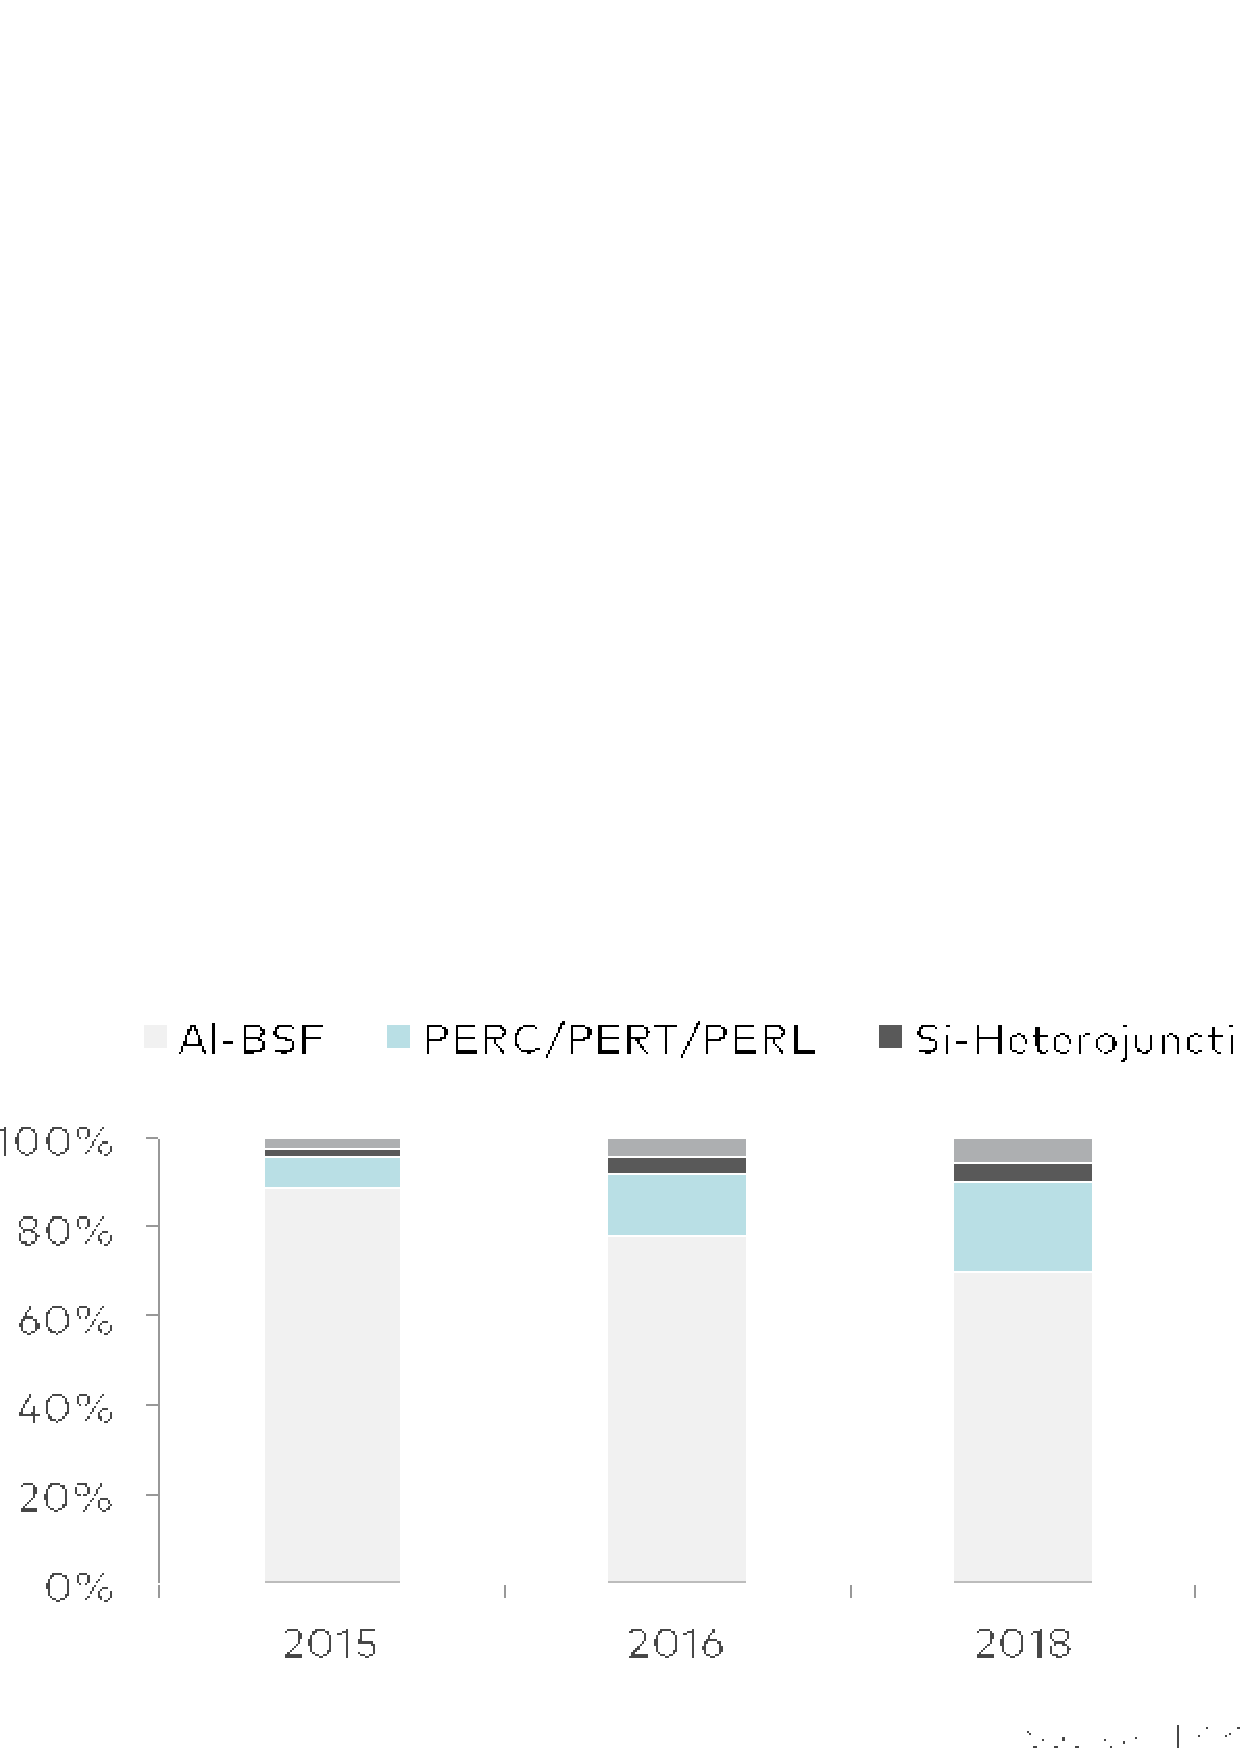
\includegraphics[width=0.48\textwidth]{BSF_PERC1}
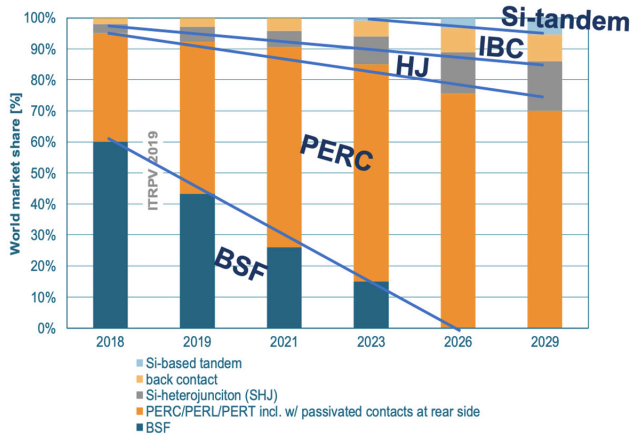
\includegraphics[width=0.48\textwidth]{BSF_PERC2}
\caption{Projected manufacturing capacity share of different
silicon--based cell technologies.
Sources:  https://www.aleo-solar.com/perc-cell-technology-explained/
(left panel), \cite{GreenRew2019} (right panel).
}
\label{fig_BSF}
\end{figure}

SCAPS-1D is a one-dimensional solar cell simulation programme and
the modeling of PERC solar cells with rear contact, which is
inhomogeneous in surface is hard task.
We understand the limitations of 1D simulators and noted about this in the Conclusion.

We agree that it would be better to use Al-doped $p^+$-layer, but please consider the following.
The simulated IV curves were used to obtain the ideality factor value $n$.
According used two-diode model,
$n$ characterizes current of second (so-called recombination)  diode;
the current of second diode current is due to recombination within
the depletion region mainly \citep{Breitenstein2013,n2McIntosh}.
The $p^+$--layer influence on mentioned process is rather determined by
pulling electric field.
Therefore the kind of doping atom in $p^+$--layer is not very important for our simulation.
In the case of $n^+-p-p^+$ structure with Al-doped base the new training data set is needed,
but the proposed deep-learning oriented approach to determining the impurity concentration remains valid.
On the other hand, the recombination in the rear surface region is not dominant
in $n$ value determination.
In our opinion, the trained DNN can be applied to PERC solar cell in which
i)~the base is boron-doped;
ii)~the iron-related deep levels are the main reason of defect-assisted recombination.


The text was revised and some speculations were added (last tree paragraph before Conclusion).


\vspace{1cm}
\noindent
\textcolor[rgb]{0.00,0.50,1.00}{\textbf{Comment~2.}}
\emph{As far as I understand, the simulation with SCAPS could be improved: emitter and BSF are uniform and this is not the case in reality.
There is no mention to the metallization, are there no contacts?
There should be, and they will influence the carrier transport and also the surface recombination velocities in the metal-semiconductor interface, among others.}

\vspace{0.5cm}
\noindent
\textcolor[rgb]{0.51,0.00,0.00}{\textbf{Reply:}}
The flat bands conditions were assumed for metal contacts on on the rear and
front surfaces.
A sentence was added in text. 
Let us note that it is common practice not to pay special attention in SCAPS simulation 
to contacts in the case of
the barrier absence --- e.g., see \cite{SCAPSuseSi4,SCAPSuseSi1,SCAPSuse1,SCAPSuse5,ScapsUse10}.



The Reviewer is correct about the way of SCAPS simulation improvement.
In the present paper, we have concentrated on recombination in the SC base region,
which mainly determine ideality factor value.
The non-uniformities of emitter and  BSF-layer affect much weaker on $n$ value.
In any case the Reviewer’s suggestion is very interesting, and must be done in the 
future. 

\vspace{1cm}
\noindent
\textcolor[rgb]{0.00,0.50,1.00}{\textbf{Comment~3.}}
\emph{Why a voltage sweep restricted to 0.45 V?
This is rather low when compared to the voltages at the maximum power point of BSF solar cells...
Wouldn't it influence in the extraction of the ideality factor values?}

\vspace{0.5cm}
\noindent
\textcolor[rgb]{0.51,0.00,0.00}{\textbf{Reply:}}
We used the two-diode model to fit the simulated data.
According to the two-diode model, the dark SC current is given by
\begin{equation}
\label{eqIVd}
    I=I_{01}\left[\exp\left(-\frac{q(V-R_sI)}{kT}\right)-1\right]
      + I_{02}\left[\exp\left(-\frac{q(V-R_sI)}{nkT}\right)-1\right]
      +\frac{V-R_sI}{R_{sh}}\,,
\end{equation}
where
$I_{01}$ and $I_{02}$ are the saturation currents,
$R_{sh}$ and $R_s$ are the shunt and series resistances.
The two-diode model is often applied for description of real Si SCs
and the first diode represents the ``ideal'' diode and
first term in Eq.~(\ref{eqIVd})
current is due to recombination in the base
and the emitter, including their surfaces;
the second diode is the so-called recombination diode
and second term is due to recombination within
the depletion region \citep{Breitenstein2013}.

\begin{figure}[t]
\centering
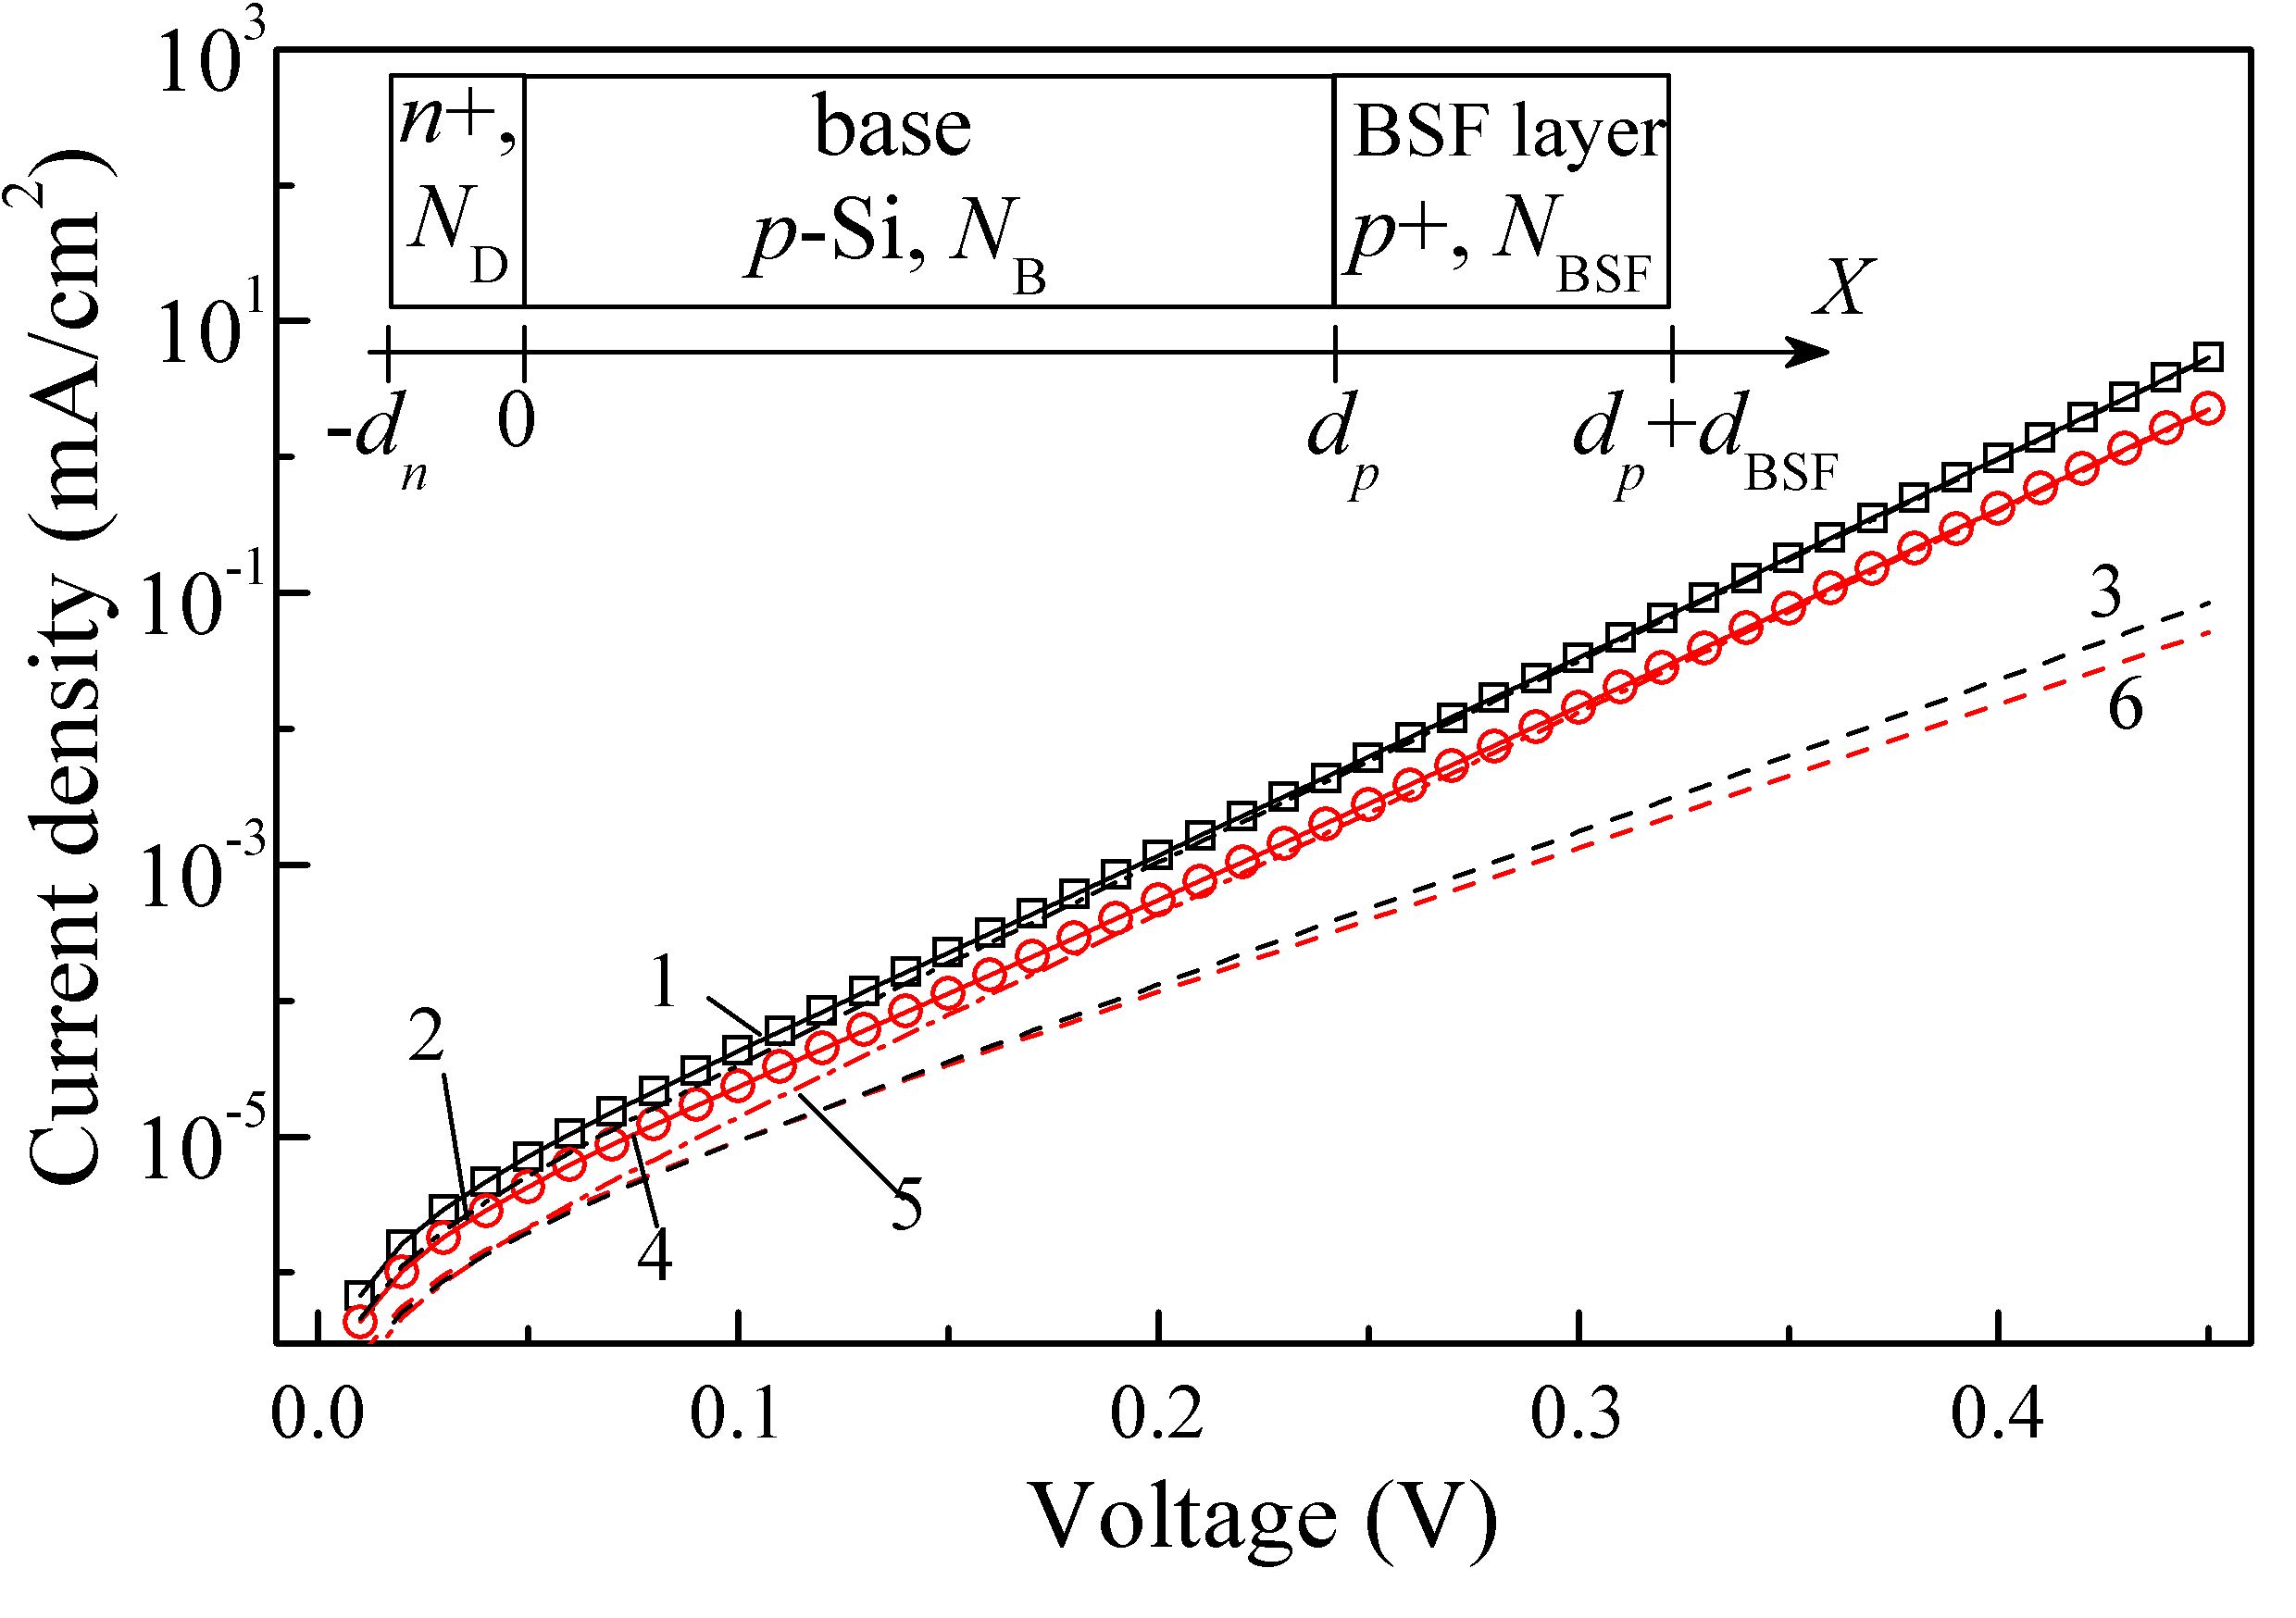
\includegraphics[width=0.5\textwidth]{FigIV}
\caption{Simulated IV characteristic (marks)
and its fitting by Eq.~(\ref{eqIVd}) (solid lines 1 and 4).
The dashed (3, 6) and dotted--dashed (2, 5)
lines represent the recombination diode currents and the ``ideal'' diode currents, respectively.
$N_\mathrm{B} = 10^{17}$~cm$^{-3}$, $N_\mathrm{Fe} = 10^{13}$~cm$^{-3}$,
$T = 340$~K, $d_p = 180$~$\mu$m.
The results for Fe-case (circles, curves 4-6, red)
and Fe-FeB case (squares, curves 1-3, black) are presented.
Inset: Structures, which are used in the simulation.
}
\label{fig_IV}
\end{figure}

The typical IV curves are shown in Fig.~\ref{fig_IV}.
It is seen that the contribution of recombination diode current is essential at low bias only.
At $V\simeq 0.25$~V the first term in Eq.~(\ref{eqIVd}) is
by an order of magnitude larger than the second one.
Similar situation is observed for
experimental IV curves --- see Fig.~9 in Manuscript.
The ideality factor value is related to slope of recombination current
dependence on voltage in semi-logarithmic scale.
Therefore the voltage range $(0-0.45)$~V is quite sufficient for an accurate determination of the ideality factor values.



The information was added in page


\vspace{1cm}
\noindent
\textcolor[rgb]{0.00,0.50,1.00}{\textbf{Comment~4.}}
\emph{I am not sure that I interpret well the results in table 5.
In the text the authors state that "the results even exceed expectations".
But what I see is that the predictions fail in general, largely for the trained dataset cases, 
but also for the full dataset.
There is some discussion on why DNN$_{FeFeB-Fe}$ performs worse than DNN$_{FeFeB}$ 
and that is Ok... but DNN$_{FeFeB}$ also fails in many cases, isn't it?
(temperatures higher than 300K for the higher Fe content, 
100\% or more error for the training dataset...).
}

\vspace{0.5cm}
\noindent
\textcolor[rgb]{0.51,0.00,0.00}{\textbf{Reply:}}
On the one hand, the Reviewer is right. 
Unfortunately the DNNs which have be trained by synthetic data 
was disable to measure iron concentration 
with extremely high precision in real solar cells 
(with a certain mismatch in their parameters and those used in the simulation).
From this point of view ``glass is half empty''.

On the other hand, the some reasons for ``glass is half full''
are present as well.
First of all, in our opinion, the 
low cost express method which use widely applied
setup and is able to approximate estimate the range of iron concentration
(even with 100\% error) can be useful.
In addition, the possible pathways for precision improving are discussed in Conclusion.
Moreover, the results in Table~5 prompt the correct utilization of proposed method in practice.
Namely the near room temperature of IV measurement is preferable;
the time between the pair dissociation and IV measurement must be as short as possible.
Finally,  

We hope that the using of deep
learning for retrieval of deep level parameters from the
current--voltage curve will find further development. 

\vspace{1cm}
\noindent
\textcolor[rgb]{0.00,0.50,1.00}{\textbf{Comment~5.}}
\emph{In the jargon, we do not talk of surface resistance, but sheet resistance.
Also, it is the first time that I read the "anti-recombination isotype barrier" for a high-low junction or a BSF.}

\vspace{0.5cm}
\noindent
\textcolor[rgb]{0.51,0.00,0.00}{\textbf{Reply:}}
The Reviewer is absolutely right.
We have revised the text accordingly. 

\vspace{1cm}
\noindent
\textcolor[rgb]{0.00,0.50,1.00}{\textbf{Comment~6.}}
\emph{It is mentioned in the paper that there is Suplementary Material, but I have not had the opportunity to read it.}

\vspace{0.5cm}
\noindent
\textcolor[rgb]{0.51,0.00,0.00}{\textbf{Reply:}}
We apologize for embarrassing.
But we are in confusion:
Reviewer \#2 mentioned about the data in the table of Supplementary Material.


\vspace{1cm}
\noindent
\textcolor[rgb]{0.00,0.50,1.00}{\textbf{Comment~7.}}
\emph{On the other hand, the paper needs a thorough revision of English, preferably by a native or bilingual speaker.
English is not my mother tongue, but I think that there are many expressions that are not correct, and make the reading difficult.
From the abstract ("The low-cost and express...", "an ideality factor values"...)
to the conclusions ("not numerous input parameters can be multiplied and transformed to the picture and apply a vision model..."(?),
and a lot in between: "both for microelectronics, logic technologies and solar cells",
"the various semiconductor barrier structures", "practical using", "Fours", "SFB", "in our further calculation",
"simulated with using", "in comparing with", "more narrow", etc. etc. }

\vspace{0.5cm}
\noindent
\textcolor[rgb]{0.51,0.00,0.00}{\textbf{Reply:}}
We are sorry for English.
The text was revised by bilingual speaker and we hope for language improving.




\subsection*{Response to Reviewer \#2 }


\textcolor[rgb]{0.00,0.50,1.00}{\textbf{Comment~1.}}
\emph{2 Simulation details}

\emph{It is assumed that all SRH recombination in the device come from iron impurities and the associated deep level defects.
It seems necessary to discuss its validity, and it could be interesting to put it against the fact that Al-BSF devices based on Czochralski silicon wafers are considered.
More generally, if another type of defects is present in the solar cell, also inducing SRH recombination,
is it possible to estimate to what extend are the DNNs trained here still accurate ? }

\vspace{0.5cm}
\noindent
\textcolor[rgb]{0.51,0.00,0.00}{\textbf{Reply:}}

The speculations about applicability of the trained DNNs to different SC structures
must be based on assumption that the ideality factor distinguishes
depletion-region recombination from most other source of recombination \cite{Breitenstein2013,n2McIntosh}.
Certainly, there are some differences from this rule for real structures.
For instance, our simulation reveals the $n$ dependence on base thickness \cite{OlikhJPS}.
But this dependence is weak and the ideality factor value is mainly determined
by depletion-region recombination nevertheless.

First of all, the DNNs applicability related to requirement of 
predominating of Shockley–Read–Hall recombination.
In the cases of other mechanism of free carrier concentration decrease the
models which diverge from two-diode is proposed (e.g., tree-diode \cite{TreeDiode,Shah}).
Moreover, the base must be doped by boron.
For example, if SC prepared from Si:Al wafer,
the simulation model which is used for training model preparing must
be modified: the parameters of $\mathrm{Fe}_i\mathrm{Al}_s$ pair are needed 
to take into consideration as well as the changes of defect 
distribution (Eq.~(\ref{eqNFeB})).
Finally, if another type of defects (in addition to iron--related deep levels)
is present in the solar cell, also inducing intensive SRH recombination,
the simulation model must be more complicated as well.
The primary competitors of $\mathrm{Fe}_i\mathrm{B}_s$  are  boron-oxygen complexes \cite{LIDRev,LIDRev2}
and oxide precipitates \cite{MurphySC2014,Oxide:Chen} in Cz-Si; 
and the corresponding model can be a next step.
By the way, it is pertinent to note that the indicator of 
the another defects presence can be a high $n$ value:
in our simulation $n<1.4$ is observed.
It is possible that last is most limiting factor of the DNNs applicability;
in particular, it confined SCs selection for experimental verification of proposed method.
 
Thus the trained DNNs can be applied to BSF solar cell prepared from Si:B wafers.
It would be noted that the modern manufacturing technique allows to substantially restrict
oxygen concentration in even Cz-Si.
On the one hand,  the Al is used to produce the doped $p^+$ region
at the industrial level \cite{GreenRew2019,WilsonRew2020}.
The $p^{+}$ layer which doped by boron was under our consideration 
(the monitoring and reproducibility of the boron diffusion from the gas phase 
$\mathrm{B}\mathrm{Cl}_3$ enable to improve SC quality)
On the other hand, the $p^+$--layer influence on depletion-region recombination
process is rather determined by pulling electric field.
Therefore the kind of doping atom in $p^+$--layer is not very important for simulation
and in our opinion the  DNNs is applicable for Al BSF cell as well.


Some speculations were added (last tree paragraph before Conclusion).


\vspace{1cm}
\noindent
\textcolor[rgb]{0.00,0.50,1.00}{\textbf{Comment~2.}}
\emph{When Fe-FeB and Fe cases are presented, it could be clearer to provide very few more explanations on both types of defects,
and the important fact that iron-boron pairs can be temporarily dissociated, providing the Fe case,
through the heat treatment or high illumination already mentioned. }

\vspace{0.5cm}
\noindent
\textcolor[rgb]{0.51,0.00,0.00}{\textbf{Reply:}}
The corresponding corrections were done in page


\vspace{1cm}
\noindent
\textcolor[rgb]{0.00,0.50,1.00}{\textbf{Comment~3.}}
\emph{3 Deep neural network models}

\emph{
It is clear how the main training dataset is created, and how the 4 * 9 * 11 * 19 = 7524 IV curves are generated.
However, the definition of the test datasets and the values for temperature,
base thickness, iron concentration and doping level are not clear for each T-varied, d-varied, etc. test set. }

\vspace{0.5cm}
\noindent
\textcolor[rgb]{0.51,0.00,0.00}{\textbf{Reply:}}
The sample of values which used for Fe-varied dataset was added in page  





\vspace{1cm}
\noindent
\textcolor[rgb]{0.00,0.50,1.00}{\textbf{Comment~4.}}
\emph{
For instance, in the case of the T-varied test set, it is mentioned that the same base thickness,
iron concentration and doping level values are used as in training dataset.
However, 4 * 9 * 19 = 684 and the amount of 894 IVs can’t be explained by multiplying with any number of temperature values.
In Supplementary Material, the associated summary table do neither explain this value 894. More generally these tables are difficult to interpret. It is possible that the subset of 144 values for T-varied test has been duplicated. }

\vspace{0.5cm}
\noindent
\textcolor[rgb]{0.51,0.00,0.00}{\textbf{Reply:}}
The Reviewer is absolutely right:
i)~the subset of 144 values for T-varied test dataset has been duplicated;
ii)~Table in Supplementary Material has a mistakes and is not clear.
The correct values of $d_p$, $N_\mathrm{B}$, and $N_{\mathrm{Fe}}$ were listed in Table,
but we have a some problems with addition and multiplication.
We apologize for the inattention.
Table in Supplementary Material was revised.

\vspace{1cm}
\noindent
\textcolor[rgb]{0.00,0.50,1.00}{\textbf{Comment~5.}}
\emph{4 Results and discussion}

\emph{
On figures 4, 5, 6 and 7, very interesting results are presented, 
and analyses of the dependence of estimation
error with temperature, boron or iron densities and base thickness are well done.
However, it seems that the same error statistics of results obtained on test datasets
(instead of training dataset) would more directly assess the quality of predictions by the DNNs.
For instance, the Fe-varied dataset has been identified to be
the closest to “real demand” or results obtained with the all-varied dataset 
would also be most probably very useful.
Such results could be showed in Supplementary Material, in the same form as figures 4, 5, 6 and 7. }

\vspace{0.5cm}
\noindent
\textcolor[rgb]{0.51,0.00,0.00}{\textbf{Reply:}}
The Supplementary Material was completed by figures (Figs.~8S--) 
which  represent similar results for test datasets.

But it would be noted that error statistics for training dataset is more correct.
In fact






%\bibliographystyle{rss}
\bibliographystyle{WileyNJD-Harvard}
\bibliography{olikh}


\end{document}
